% questions.tex —— 2007 年·普通高等学校招生考试·浙江卷·理科 · 题目内容片段（无答案）
% 由 tools/generate_projects.py 依来源总账自 2007/2007_数学真题_浙江理_试题.md 生成，勿手改（改源 MD 后重跑）


\gkpart{一、选择题}

\begin{question}
\gkti{1}“$x>1$”是“$x^2>x$”的（　）

（A）充分而不必要条件

（B）必要而不充分条件

（C）充分必要条件

（D）既不充分也不必要条件

\end{question}
\begin{question}
\gkti{2}若函数 $f(x)=2\sin(\omega x+\varphi)$，$x\in\mathbf R$（其中 $\omega>0$，$|\varphi|<\dfrac{\pi}{2}$）的最小正周期是 $\pi$，且 $f(0)=\sqrt3$，则（　）

（A）$\omega=\dfrac12$，$\varphi=\dfrac{\pi}{6}$

（B）$\omega=\dfrac12$，$\varphi=\dfrac{\pi}{3}$

（C）$\omega=2$，$\varphi=\dfrac{\pi}{6}$

（D）$\omega=2$，$\varphi=\dfrac{\pi}{3}$

\end{question}
\begin{question}
\gkti{3}直线 $x-2y+1=0$ 关于直线 $x=1$ 对称的直线方程是（　）

（A）$x+2y-1=0$

（B）$2x+y-1=0$

（C）$2x+y-3=0$

（D）$x+2y-3=0$

\Needspace{0.4\textheight}
\end{question}
\begin{question}
\gkti{4}要在边长为 $16$ 米的正方形草坪上安装喷水龙头，使整个草坪都能喷洒到水。假设每个喷水龙头的喷洒范围都是半径为 $6$ 米的圆面，则需安装这种喷水龙头的个数最少是（　）
\nopagebreak[4]
\begin{center}% 2007 年浙江卷理科第 4 题：边长 16 米的正方形草坪与喷水龙头示意。
% 来源 PDF：gaokaomath-src/普通高考/2007/2007浙江理.pdf
% SHA-256：31c1d0d79ba11a3644a27b5ee3781f52caaf831209e8da63ddd8d7019cd06995
% 原页：2007浙江理.pdf 第 1 页（A3 三栏）第 1 栏，书页码 417。
% 重绘依据：按原页正方形草坪与中心喷水圆面的透视重绘。
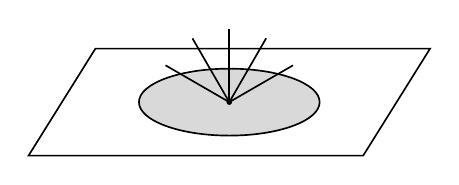
\begin{tikzpicture}[scale=0.85, semithick,
  every node/.style={inner sep=1pt}]

  % 正方形草坪（斜投影）
  \draw (0,0) -- (5,0) -- (6,1.6) -- (1,1.6) -- cycle;

  % 喷水圆面
  \fill[gray!30] (3,0.8) ellipse (1.35 and 0.5);
  \draw (3,0.8) ellipse (1.35 and 0.5);
  \fill (3,0.8) circle (1.2pt);

  % 水花射线
  \foreach \a in {30,60,90,120,150} {
    \draw (3,0.8) -- ++(\a:1.1);
  }
\end{tikzpicture}
\end{center}
\nopagebreak[4]
（A）$3$

（B）$4$

（C）$5$

（D）$6$

\end{question}
\begin{question}
\gkti{5}已知随机变量 $\xi$ 服从正态分布 $N(2,\sigma^2)$，$P(\xi\leqslant4)=0.84$，则 $P(\xi\leqslant0)=$（　）

（A）$0.16$

（B）$0.32$

（C）$0.68$

（D）$0.84$

\end{question}
\begin{question}
\gkti{6}若 $P$ 是两条异面直线 $l$，$m$ 外的任意一点，则（　）

（A）过点 $P$ 有且仅有一条直线与 $l$，$m$ 都平行

（B）过点 $P$ 有且仅有一条直线与 $l$，$m$ 都垂直

（C）过点 $P$ 有且仅有一条直线与 $l$，$m$ 都相交

（D）过点 $P$ 有且仅有一条直线与 $l$，$m$ 都异面

\end{question}
\begin{question}
\gkti{7}若非零向量 $\boldsymbol a$，$\boldsymbol b$ 满足 $|\boldsymbol a+\boldsymbol b|=|\boldsymbol b|$，则（　）

（A）$|2\boldsymbol a|>|2\boldsymbol a+\boldsymbol b|$

（B）$|2\boldsymbol a|<|2\boldsymbol a+\boldsymbol b|$

（C）$|2\boldsymbol b|>|\boldsymbol a+2\boldsymbol b|$

（D）$|2\boldsymbol b|<|\boldsymbol a+2\boldsymbol b|$

\Needspace{0.4\textheight}
\end{question}
\begin{question}
\gkti{8}设 $f'(x)$ 是函数 $f(x)$ 的导函数，将 $y=f(x)$ 和 $y=f'(x)$ 的图象画在同一个直角坐标系中，不可能正确的是（　）
\nopagebreak[4]
\begin{center}% 2007 年浙江卷理科第 8 题：y=f(x) 与 y=f'(x) 在同一坐标系中的四个图象选项。
%   （A）f=x^2 与 f'=2x；（B）f 单调递减而 f' 取正值（不可能）；
%   （C）f=e^x 与 f'=e^x；（D）f 为四次型曲线、f' 在其极值点变号。
% 来源 PDF：gaokaomath-src/普通高考/2007/2007浙江理.pdf
% SHA-256：3b1e5fbca7888b1cff1fc809211aac94f14ea503de0229c4edf7cfb54e5bd2d4
% 原页：2007浙江理.pdf 第 1 页（A3 三栏）第 2 栏，书页码 417。
% 重绘依据：按原页四个小图的曲线形状、相对位置与坐标轴重绘。
\begin{tikzpicture}[scale=0.9, semithick,
  every node/.style={inner sep=1pt, font=\small}]

  % ---------------- （A） ----------------
  \begin{scope}[shift={(0,0)}]
    \draw[->,>=stealth] (-1.8,0) -- (2.1,0) node[right] {$x$};
    \draw[->,>=stealth] (0,-1.4) -- (0,1.8) node[above] {$y$};
    \draw[domain=-1.25:1.25,samples=100] plot (\x,{\x*\x});
    \draw (-1.5,-1.2) -- (1.5,1.2);
    \node[below] at (0.8,-1.7) {（A）};
  \end{scope}

  % ---------------- （B） ----------------
  \begin{scope}[shift={(4.6,0)}]
    \draw[->,>=stealth] (-1.8,0) -- (2.1,0) node[right] {$x$};
    \draw[->,>=stealth] (0,-1.4) -- (0,1.8) node[above] {$y$};
    \draw[domain=-1.4:1.4,samples=100] plot (\x,{1.3*exp(-0.7*(\x+0.2))});
    \draw[domain=-1.4:1.4,samples=100] plot (\x,{0.9*(\x-0.1)});
    \node[below] at (0.8,-1.7) {（B）};
  \end{scope}

  % ---------------- （C） ----------------
  \begin{scope}[shift={(0,-4.4)}]
    \draw[->,>=stealth] (-1.8,0) -- (2.1,0) node[right] {$x$};
    \draw[->,>=stealth] (0,-1.4) -- (0,1.8) node[above] {$y$};
    \draw[domain=-1.3:0.55,samples=100] plot (\x,{0.55*exp(1.1*\x)});
    \draw[domain=-0.2:1.2,samples=100] plot (\x,{0.65*exp(0.8*\x)});
    \node[below] at (0.8,-1.7) {（C）};
  \end{scope}

  % ---------------- （D） ----------------
  \begin{scope}[shift={(4.6,-4.4)}]
    \draw[->,>=stealth] (-1.8,0) -- (2.1,0) node[right] {$x$};
    \draw[->,>=stealth] (0,-1.4) -- (0,1.8) node[above] {$y$};
    \draw[domain=-1.4:1.5,samples=120]
      plot (\x,{0.9*cos(deg(2.2*\x))});
    \draw[domain=-1.4:1.5,samples=120]
      plot (\x,{0.55*sin(deg(2.2*\x))});
    \node[below] at (0.8,-1.7) {（D）};
  \end{scope}
\end{tikzpicture}
\end{center}
\nopagebreak[4]
\end{question}
\begin{question}
\gkti{9}已知双曲线 $\dfrac{x^2}{a^2}-\dfrac{y^2}{b^2}=1$（$a>0$，$b>0$）的左、右焦点分别为 $F_1$，$F_2$，$P$ 是准线上一点，且 $PF_1\perp PF_2$，$|PF_1|\cdot|PF_2|=4ab$，则双曲线的离心率是（　）

（A）$\sqrt2$

（B）$\sqrt3$

（C）$2$

（D）$3$

\end{question}
\begin{question}
\gkti{10}设 $f(x)=\begin{cases}x^2,&|x|\geqslant1,\\ x,&|x|<1,\end{cases}$ 若 $f(g(x))$ 的值域是 $[0,+\infty)$，则函数 $g(x)$ 的值域是（　）

（A）$(-\infty,-1]\cup[1,+\infty)$

（B）$(-\infty,-1]\cup[0,+\infty)$

（C）$[0,+\infty)$

（D）$[1,+\infty)$

\end{question}
\gkpart{二、填空题}

\begin{question}
\gkti{11}已知复数 $z_1=1-\mathrm i$，$z_1\cdot z_2=1+\mathrm i$，则复数 $z_2=$\gkblank{}。

\end{question}
\begin{question}
\gkti{12}已知 $\sin\theta+\cos\theta=\dfrac15$，且 $\dfrac{\pi}{2}\leqslant\theta\leqslant\dfrac{3\pi}{4}$，则 $\cos2\theta$ 的值是\gkblank{}。

\end{question}
\begin{question}
\gkti{13}不等式 $|2x-1|-x<1$ 的解集是\gkblank{}。

\end{question}
\begin{question}
\gkti{14}某书店有 $11$ 种杂志，$2$ 元 $1$ 本的 $8$ 种，$1$ 元 $1$ 本的 $3$ 种。小张用 $10$ 元钱买杂志（每种至多买一本，$10$ 元钱刚好用完），则不同买法的种数是\gkblank{}。（用数字作答）

\end{question}
\begin{question}
\gkti{15}随机变量 $\xi$ 的分布列如下：

\begin{center}
\begin{tabular}{llll}
\toprule
$\xi$ & $-1$ & $0$ & $1$ \\
\midrule
$P$ & $a$ & $b$ & $c$ \\
\bottomrule
\end{tabular}
\end{center}

其中 $a$，$b$，$c$ 成等差数列。若 $E\xi=\dfrac13$，则 $D\xi$ 的值是\gkblank{}。

\end{question}
\begin{question}
\gkti{16}已知点 $O$ 在二面角 $\alpha-AB-\beta$ 的棱上，点 $P$ 在 $\alpha$ 内，且 $\angle POB=45^\circ$。若对于 $\beta$ 内异于 $O$ 的任意一点 $Q$，都有 $\angle POQ\geqslant45^\circ$，则二面角 $\alpha-AB-\beta$ 的大小是\gkblank{}。

\end{question}
\begin{question}
\gkti{17}设 $m$ 为实数，若 $\left\{(x,y)\ \middle|\ \begin{cases}x-2y+5\geqslant0,\\ 3-x\geqslant0,\\ mx+y\geqslant0\end{cases}\right\}\subseteq\{(x,y)\mid x^2+y^2\leqslant25\}$，则 $m$ 的取值范围是\gkblank{}。

\end{question}
\gkpart{三、解答题}

\begin{question}
\gkti{18}已知 $\triangle ABC$ 的周长为 $\sqrt2+1$，且 $\sin A+\sin B=\sqrt2\sin C$。

（1）求边 $AB$ 的长；

（2）若 $\triangle ABC$ 的面积为 $\dfrac16\sin C$，求角 $C$ 的度数。

\Needspace{0.4\textheight}
\end{question}
\begin{question}
\gkti{19}在如图所示的几何体中，$EA\perp$ 平面 $ABC$，$DB\perp$ 平面 $ABC$，$AC\perp BC$，且 $AC=BC=BD=2AE$，$M$ 是 $AB$ 的中点。

（1）求证：$CM\perp EM$；

（2）求 $CM$ 与平面 $CDE$ 所成的角。
\nopagebreak[4]
\begin{center}% 2007 年浙江卷理科第 19 题：EA、DB 均垂直于平面 ABC，AC⊥BC，M 为 AB 中点。
%   按 AC=BC=2、AE=1、BD=2 的示意比例绘制。
% 来源 PDF：gaokaomath-src/普通高考/2007/2007浙江理.pdf
% SHA-256：31c1d0d79ba11a3644a27b5ee3781f52caaf831209e8da63ddd8d7019cd06995
% 原页：2007浙江理.pdf 第 2 页（A3 三栏）第 1 栏，书页码 418。
% 重绘依据：按原页 C、A、B 底面与 E、D 的竖直位置重绘。
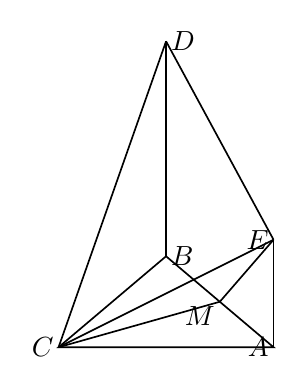
\begin{tikzpicture}[scale=1.05, semithick,
  every node/.style={inner sep=1.5pt}]

  \coordinate (C) at (0,0);
  \coordinate (A) at (2.6,0);
  \coordinate (B) at (1.3,1.1);
  \coordinate (E) at (2.6,1.3);
  \coordinate (D) at (1.3,3.7);
  \coordinate (M) at (1.95,0.55);

  % 底面
  \draw (C) -- (A) -- (B) -- cycle;
  % 竖直线
  \draw (A) -- (E);
  \draw (B) -- (D);
  % 上方连线
  \draw (E) -- (D);
  \draw (E) -- (C);
  \draw (D) -- (C);
  % 中点 M 相关
  \draw (C) -- (M);
  \draw (E) -- (M);

  \node[left] at (C) {$C$};
  \node[left] at (A) {$A$};
  \node[right] at (B) {$B$};
  \node[left] at (E) {$E$};
  \node[right] at (D) {$D$};
  \node[below left] at (M) {$M$};
\end{tikzpicture}
\end{center}
\nopagebreak[4]
\Needspace{0.4\textheight}
\end{question}
\begin{question}
\gkti{20}如图，直线 $y=kx+b$ 与椭圆 $\dfrac{x^2}{4}+y^2=1$ 交于 $A$，$B$ 两点，记 $\triangle AOB$ 的面积为 $S$。

（1）求在 $k=0$，$0<b<1$ 的条件下，$S$ 的最大值；

（2）当 $|AB|=2$，$S=1$ 时，求直线 $AB$ 的方程。
\nopagebreak[4]
\begin{center}% 2007 年浙江卷理科第 20 题：直线 y=kx+b 与椭圆 x^2/4+y^2=1 交于 A、B，
%   记三角形 AOB 的面积为 S。
% 来源 PDF：gaokaomath-src/普通高考/2007/2007浙江理.pdf
% SHA-256：31c1d0d79ba11a3644a27b5ee3781f52caaf831209e8da63ddd8d7019cd06995
% 原页：2007浙江理.pdf 第 2 页（A3 三栏）第 2 栏，书页码 418。
% 重绘依据：按原页椭圆、割线与 A、B、O 的位置重绘。
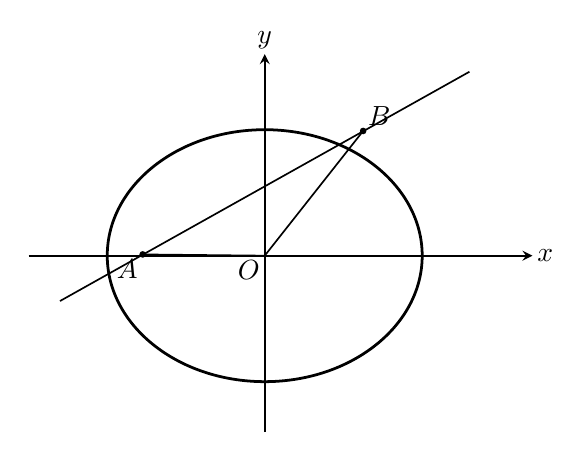
\begin{tikzpicture}[x=1.0cm, y=1.6cm, semithick,
  every node/.style={inner sep=1.5pt}]

  \draw[->,>=stealth] (-3.0,0) -- (3.4,0) node[right] {$x$};
  \draw[->,>=stealth] (0,-1.4) -- (0,1.6) node[above] {$y$};
  \node[below left] at (0,0) {$O$};

  % 椭圆 x^2/4+y^2=1
  \draw[line width=1pt] (0,0) ellipse (2 and 1);

  % 割线 y = 0.35x + 0.55（示意）
  \draw (-2.6,-0.36) -- (2.6,1.46);
  \coordinate (A) at (-1.55,0.01);
  \coordinate (B) at (1.25,0.99);
  \fill (A) circle (1.2pt);
  \fill (B) circle (1.2pt);
  \node[below left] at (A) {$A$};
  \node[above right] at (B) {$B$};

  \draw (A) -- (0,0) -- (B);
\end{tikzpicture}
\end{center}
\nopagebreak[4]
\end{question}
\begin{question}
\gkti{21}已知数列 $\{a_n\}$ 中的相邻两项 $a_{2k-1}$，$a_{2k}$ 是关于 $x$ 的方程 $x^2-(3k+2^k)x+3k\cdot2^k=0$ 的两个根，且 $a_{2k-1}\leqslant a_{2k}$（$k=1,2,3,\cdots$）。

（1）求 $a_1$，$a_3$，$a_5$，$a_7$；

（2）求数列 $\{a_n\}$ 的前 $2n$ 项和 $S_{2n}$；

（3）记 $f(n)=\dfrac12\left(\dfrac{|\sin n|}{\sin n}+3\right)$，$T_n=\dfrac{(-1)^{f(2)}}{a_1a_2}+\dfrac{(-1)^{f(3)}}{a_3a_4}+\dfrac{(-1)^{f(4)}}{a_5a_6}+\cdots+\dfrac{(-1)^{f(n+1)}}{a_{2n-1}a_{2n}}$，求证：$\dfrac16\leqslant T_n\leqslant\dfrac5{24}$（$n\in\mathbf N^*$）。

\end{question}
\begin{question}
\gkti{22}设 $f(x)=\dfrac{x^3}{3}$，对任意实数 $t$，记 $g_t(x)=t^2x-\dfrac23t^3$。

（1）求函数 $y=f(x)-g_8(x)$ 的单调区间；

（2）求证：

① 当 $x>0$ 时，$f(x)\geqslant g_t(x)$ 对任意实数 $t$ 成立；

② 有且仅有一个正实数 $x_0$，使得 $g_8(x_0)\geqslant g_t(x_0)$ 对任意实数 $t$ 成立。

\end{question}